\chapter{Planificación y presupuesto del proyecto}\label{ch:planificacion-y-presupuesto}

En esta sección se incluyen los aspectos relativos a la planificación del proyecto. Esta se divide en tres partes:
preparación inicial, desarrollo y conclusión. Cada una de estas partes representa una \textit{milestone} del proyecto
que se han realizado organizadas en \textit{sprints} de duración de dos semanas con el fin de poder llevar un control de las tareas realizadas
y alcanzar los objetivos previstos: \\

\textbf{Sprint 1: 1 de febrero - 14 de febrero}: preparación del proyecto. En este \textit{sprint} se abordan tareas únicamente
de la primera \textit{milestone}:

\begin{itemize}
    \item Creación de los repositorios
    \item Creación de la estructura inicial de los repositorios
    \item Creación de la estructura inicial de la memoria
\end{itemize}

\textbf{Sprint 2: 15 de febrero - 28 de febrero}: primeros pasos en la documentación. En este \textit{sprint} se pretende
avanzar en la documentación del proyecto de cara a cumplimentar la historia de usuario asociada a la primera \textit{milestone}:
\textbf{Como lector quiero poder conocer las bases del proyecto de manera clara y ordenada a partir de la documentación proporcionada}:
\begin{itemize}
    \item Motivación y contexto
    \item Estado del arte
\end{itemize}

\newpage

\textbf{Sprint 3: 1 de marzo - 14 de marzo}: requisitos del proyecto. En este \textit{sprint} se pretende establecer
los objetivos del proyecto una vez conociendo el contexto y el estado del arte y comenzar a definir los requisitos
del mismo:

\begin{itemize}
    \item Objetivos del proyecto
    \item Requisitos funcionales
    \item Requisitos no funcionales
\end{itemize}

\textbf{Sprint 4: 15 de marzo - 28 de marzo}: diseño del proyecto. En este \textit{sprint} se pretende comenzar a
diseñar el proyecto a partir de los requisitos establecidos en el \textit{sprint} anterior incluyendo las
tecnologías a utilizar:

\begin{itemize}
    \item Arquitectura del proyecto
    \item Diseño de la \textbf{API}
    \item Diseño de la base de datos
    \item Diseño de la aplicación web
\end{itemize}

\textbf{Sprint 5: 29 de marzo - 11 de abril}: implementación de la \textbf{API}. En este \textit{sprint} se pretende comenzar
con la implementación de la \textbf{API} y por tanto a cumplimentar diferentes tareas asociadas a la segunda \textit{milestone}:
\textbf{Gestión de animales en adopción}:

\begin{itemize}
    \item CRUD de animales
    \item CRUD de usuarios
    \item CRUD de organizaciones
    \item CRUD de peticiones de adopción
\end{itemize}

\textbf{Sprint 6: 12 de abril - 25 de abril}: implementación de la \textbf{API}. En este \textit{sprint} se pretende continuar
con la implementación de la \textbf{API}:

\begin{itemize}
    \item Registro y login de usuarios
    \item Registro y login de organizaciones
    \item Funcionalidad de reestablecimiento de contraseña
    \item Gestión de fotos de animales, usuarios y organizaciones
\end{itemize}

\textbf{Sprint 7: 26 de abril - 9 de mayo}: implementación de la \textbf{API}. En este \textit{sprint} se pretende finalizar
con la implementación de las tareas asociadas a la segunda \textit{milestone}:

\begin{itemize}
    \item Gestión de peticiones de adopción
    \item Visualización y filtrado de búsqueda de animales
\end{itemize}

\textbf{Sprint 8: 10 de mayo - 23 de mayo}: implementación de \textit{tests} y despliegues. En este \textit{sprint}
se pretende realizar la implementación de los \textit{tests} de la \textbf{API} y realizar el despliegue de la misma.

\textbf{Sprint 9: 24 de mayo - 6 de junio}: finalización de \textit{tests} e inicio de página web. En este \textit{sprint}
se pretende finalizar con la implementación de los \textit{tests} de la \textbf{API} y comenzar con la implementación de la página web.

\textbf{Sprint 10: 7 de junio - 20 de junio}: finalización de página web y despliegues. En este \textit{sprint} se pretende
dejar finalizados los despliegues de la \textbf{API} y la página web, comprobar su correcto funcionamiento y realizar los ajustes
necesarios. Se cierra a su vez la segunda \textit{milestone} del proyecto.

\textbf{Sprint 11: 21 de junio - 4 de julio}: finalización de la documentación y entrega del proyecto. En este \textit{sprint} se
pretende finalizar con la documentación del proyecto y realizar la entrega del mismo. Se cierra a su vez la tercera y
última \textit{milestone} del proyecto: \textbf{Conclusión}:

\begin{itemize}
    \item Cierre de tareas pendientes
    \item Conclusiones y finalización de la documentación
    \item Entrega del proyecto
\end{itemize}

\newpage

Durante los diferentes \textit{sprints} se han ido resolviendo las dudas presentadas con el tutor del proyecto
y se han completado los apartados correspondientes de la documentación en cada fase realizada. \\

En la siguiente tabla se muestra un resumen de las tareas en la
que se incluye el tiempo estimado para cada una de ellas:

\begin{table}[!ht]
  \centering
  \begin{tabular}{|l|l|}
    \hline
    \textbf{Tarea} & \textbf{Tiempo (horas)} \\
    \hline
    Planificación del proyecto & 90 \\
    Diseño de la API & 50 \\
    Implementación de la API & 150 \\
    Pruebas de la API & 50 \\
    Diseño de la página web & 20 \\
    Implementación de la página web & 50 \\
    Pruebas de la página web & 20 \\
    Diseño de la base de datos & 10 \\
    Pruebas de la base de datos & 20 \\
    Conclusiones & 10 \\
    \hline
    Total & 470 \\
    \hline
  \end{tabular}
  \caption{Planificación del proyecto}
  \label{tab:planificacion}
\end{table}

\newpage

\section{Diagrama de Gantt}\label{sec:diagrama-de-gantt}

El Diagrama de Gantt se usa para representar las tareas que se deben realizar en un proyecto, así como las fechas
en las que se deben realizar. En la siguiente figura se muestra el diagrama de Gantt del proyecto en el que, de forma
visual y clara, se puede ver la planificación de las tareas mencionadas anteriormente: \\

\begin{figure}[H]
    \centering
    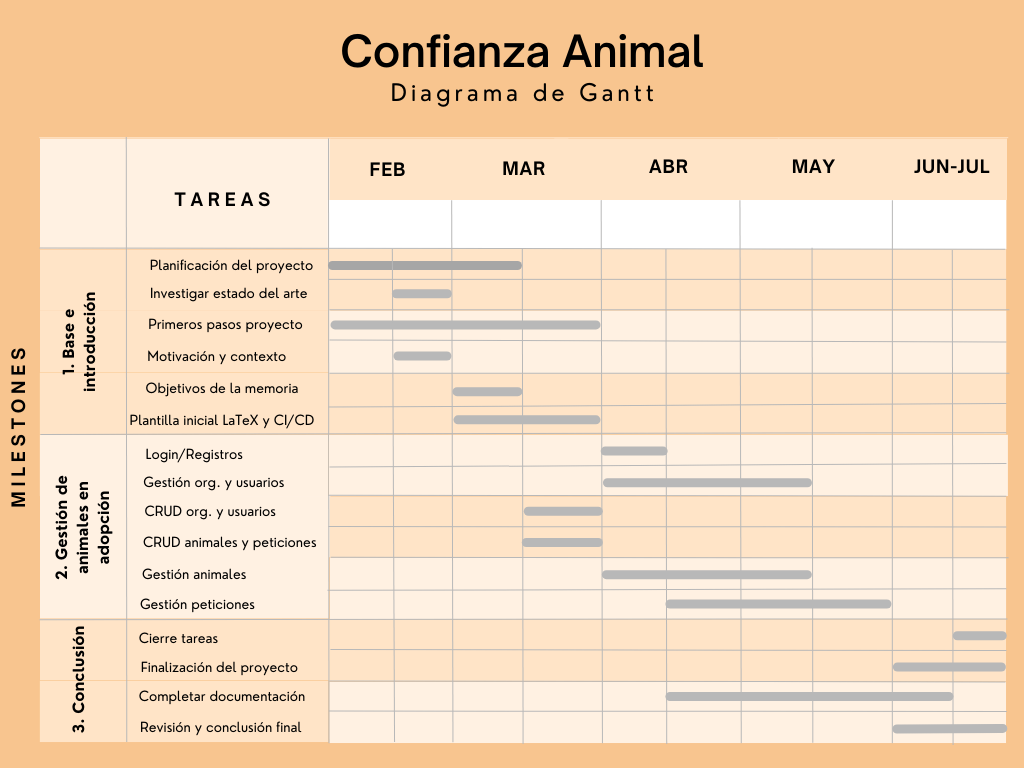
\includegraphics[width=\textwidth]{imgs/gantt}
    \caption{Diagrama de Gantt}
    \label{fig:diagrama-gantt}
\end{figure}

\newpage

\section{Elección de herramientas y tecnologías}\label{sec:eleccion-de-herramientas-y-tecnologias}

Antes de comenzar con el desarrollo del proyecto es necesario elegir las herramientas y tecnologías que se van a
utilizar para llevar a cabo el mismo. Para ello se han tenido en cuenta los requisitos del proyecto así como su
planificación y se ha llevado a cabo una investigación de las diferentes herramientas y tecnologías
existentes para cada una de las partes del proyecto que ha permitido elegir las más apropiadas para el desarrollo
del proyecto. Esto también nos ayudará a la hora de realizar la estimación de los costes del proyecto que se
explican en profundidad en la siguiente sección \ref{sec:presupuesto}.

\subsection{Framework web de API}\label{subsec:framework-web-de-api}

Para el desarrollo de la API se ha elegido \textbf{FastAPI}. Este framework por medio del lenguaje
de programación \textbf{Python} permite crear APIs de forma rápida y sencilla. Los motivos por los que
se ha elegido son los siguientes:

\begin{itemize}
    \item Es un framework moderno y rápido. El motivo de su alto rendimiento se debe a que hace uso de un sistema
    de tipado estático y un enfoque basado en declaraciones.
    \item Permite realizar operaciones de forma asíncrona. Gracias a la librería estándar \textbf{asyncio} permite que
    la API pueda realizar múltiples operaciones al mismo tiempo y de forma concurrente sin bloquear el hilo principal
    de ejecución dando una mayor velocidad de respuesta y escalabilidad.
    \item Permite realizar validaciones de datos. Por medio de la librería \textbf{Pydantic} se pueden
    validar y serializar los datos de forma automática aportando una mayor velocidad de ejecución y seguridad a la API.
    \item Permite realizar documentación de la API. FastAPI genera automáticamente una documentación interactiva
    basada en \textbf{OpenAPI} y \textbf{SwaggerUI} que facilita las pruebas de la API y la comprensión de la misma.
    \item Permite realizar la conexión con la base de datos. Uno de los puntos más importantes a la hora de elegir un
    framework es la facilidad de conexión con la base de datos. Debido a que su lenguaje de programación es \textbf{Python}
    y a día de hoy es uno de los lenguajes más utilizados en el mundo, la comunidad de desarrolladores ha creado
    una gran cantidad de librerías que permiten realizar conexiones con diferentes bases de datos. En este proyecto se ha
    usado la librería \textbf{Pyrebase}, que facilita la conexión con \textbf{Firebase} y permite realizar operaciones
    básicas como la autenticación, el almacenamiento de archivos, etc.
\end{itemize}

La gran cantidad de ventajas que ofrece \textbf{FastAPI} junto a su fácil aprendizaje sumado al interés personal
por aprender un nuevo framework hace que sea una de las mejores opciones para el desarrollo de este proyecto
frente a otras más comunes como pueden ser \textbf{Django} o \textbf{Flask}.

\subsection{Framework web de página web}\label{subsec:framework-web-de-pagina-web}

Para el desarrollo de la página web se ha elegido \textbf{Angular} en su versión 15 junto con \textbf{TypeScript}.
Angular es uno de los frameworks más utilizados en la actualidad para el desarrollo de aplicaciones web. Fue creado
por Google y su alta popularidad se debe a que es un framework muy robusto y escalable. Está basado en el patrón
de diseño \textbf{MVC} y permite realizar aplicaciones web de forma rápida y sencilla. \\

Pensando en el largo plazo, Angular es una de las mejores opciones posibles para el desarrollo de este proyecto. Cada 6 meses
Google aparece con una nueva versión que aporta nuevas características y mejoras, sigue una
arquitectura modular basada en componentes lo que proporciona una gran robustez, escalabilidad y mantenibilidad. El hecho
de que sea un framework de código abierto y que su comunidad sea muy activa hace que sea muy sencillo encontrar
soluciones a los problemas que se puedan presentar o componentes que se puedan reutilizar. \\

Angular necesita de un lenguaje de programación que se compile a JavaScript para poder
funcionar. En este proyecto se ha utilizado \textbf{TypeScript} ya que es un lenguaje que cumple con el requisito y además
tiene la peculiaridad de que es tipado estáticamente. Esto significa que el compilador de TypeScript comprueba que los
tipos de datos de las variables y funciones son correctos proporcionando así una mayor robustez y seguridad al código. \\

En los siguientes subapartados se mencionan en mayor profundidad los \textit{frameworks} CSS y bibliotecas empleadas que
han facilitado el diseño y creación de componentes de la página web como son \textbf{Angular Material}, \textbf{Bootstrap} y \textbf{Tailwind CSS}:

\subsubsection{Angular Material}\label{subsubsec:angular-material}

Angular Material es una biblioteca de componentes de diseño de código abierto para Angular que proporciona
una gran cantidad de componentes reutilizables y que ayudan a crear interfaces de usuario atractivas y funcionales. \\

Se basa en el diseño Material Design de Google, centrada en la simplicidad y la legibilidad. Entre su amplia gama de
componentes predefinidos se encuentran botones, barras de navegación, menús, listas, cuadros de diálogo, tablas, etc. \\

Algunas de las razones por las que se ha elegido Angular Material son:

\begin{itemize}
    \item \textbf{Responsive}: los componentes de Angular Material se adaptan a los diferentes tamaños de pantalla
    de forma automática y sin necesidad de escribir código adicional para ello.
    \item \textbf{Fácil de usar}: los componentes son muy fáciles de implementar y de usar ya que se basan en
    directivas de Angular y se pueden personalizar fácilmente mediante clases CSS y atributos.
    \item \textbf{Personalizable}: al ser código abierto, se puede ver el código fuente de los componentes y
    modificarlos a nuestro gusto para adaptarlos a nuestras necesidades.
    \item \textbf{Documentación}: la documentación de Angular Material es muy completa y detallada, además
    de que cuenta con ejemplos de uso de cada componente.
    \item \textbf{Accesibilidad}: los componentes de Angular Material cumplen con las normas de accesibilidad W3C~\cite{W3C} y
    están diseñados para que sean usados por personas con discapacidad visual, auditiva o motora.
\end{itemize}

\subsubsection{Bootstrap}\label{subsubsec:bootstrap}

Bootstrap es a día de hoy uno de los frameworks de CSS más populares y utilizados. Es un framework de código abierto
que permite la creación de interfaces de usuario \textit{responsive} por medio de componentes predefinidos, de
la misma forma que ocurre con Angular Material. \\

Usar Bootstrap junto a Angular Material ha permitido una serie de ventajas adicionales para el proyecto:

\begin{itemize}
    \item \textbf{Mayor variedad de componentes}: al combinar los componentes de Angular Material con los de Bootstrap,
    se ha conseguido una mayor variedad para la creación de las interfaces de usuario.
    \item \textbf{Ahorro de tiempo}: de la mano del punto anterior, el hecho de contar con un amplia gama de componentes predefinidos,
    se ha ahorrado tiempo en la creación de los componentes de la página web desde cero.
    \item \textbf{Compatibilidad}: Bootstrap asegura que sus componentes funcionan correctamente con los diferentes
    navegadores y dispositivos, lo cual garantiza una mayor experiencia de usuario y una interfaz más consistente.
    \item \textbf{Estilos por defecto}: Bootstrap cuenta con una gran cantidad de estilos CSS que permiten la personalización
    de los componentes de forma sencilla y rápida. Un ejemplo de esto podría ser la clase de estilo \texttt{mr-2} que
    añade automáticamente un margen a la derecha de 2 unidades a un elemento en vez de tener que escribir el código CSS correspondiente.
\end{itemize}

\subsubsection{Tailwind CSS}\label{subsubsec:tailwind-css}

Tailwind CSS es un framework de diseño web que se centra mayormente en proporcionar una amplia gama de clases CSS
personalizables para ayudar a crear interfaces de usuario de forma rápida y sencilla. A diferencia de Bootstrap, que
ya hemos viso que ofrece estilos predefinidos para los componentes, Tailwind CSS no proporciona ningún estilo por defecto,
sino que se basa en clases CSS que se pueden combinar para crear estilos personalizados. \\

Uno de los principales motivos por los que se ha añadido Tailwind CSS al proyecto es para probar un framework
moderno y que se está empezando a popularizar. Además, se ha elegido por su facilidad de uso, por la gran cantidad
de clases CSS que ofrece y por reducir las líneas de código CSS que se pueden llegar a escribir en un proyecto de
esta envergadura.

\subsection{Base de datos no relacional}\label{subsec:base-de-datos-no-relacional}

Para el almacenamiento de datos se ha elegido la base de datos de \textbf{Firebase}. Esta base de datos, tal y como
indica el apartado, es no relacional y se basa en colecciones y documentos. Cada documento es un objeto JSON que
contiene una serie de pares clave-valor. Los documentos se almacenan en colecciones que son como tablas en una base de datos
relacional. \\

Las bases de datos no relacionales, también conocidas como \textbf{NoSQL} se caracterizan por no tener que definir un
esquema de datos fijo previamente en el que se relacionen entre sí por medio de claves primarias o foráneas tal y
como ocurre en las bases de datos relacionales. Esto hace que las bases de datos no relacionales sean más flexibles
y escalables y no requieran de grandes consultas para obtener los datos. \\

Para este proyecto este tipo de base de datos es ideal ya que los animales pueden tener diferentes características
y sea necesario modificar el esquema de datos en cualquier momento. Además, se espera trabajar con una gran cantidad
de información e imágenes que requieren de un gran almacenamiento y para estos casos las bases de datos no relacionales
que escalan horizontalmente ofrecen un gran rendimiento en la lectura y escritura de datos. \\

En el siguiente subapartado se explicará con más detalle las características de \textbf{Firebase} y los motivos por
los que se ha elegido esta base de datos:

\subsubsection{Firebase}\label{subsubsec:firebase}
Firebase es una plataforma de Google que ofrece una amplia gama de servicios
para desarrollar aplicaciones web y móviles de una forma rápida, eficiente y de alta calidad. \\

La base de datos propia de Firebase es una base de datos no relacional que permite almacenar datos en forma de documentos JSON,
realizar consultas en tiempo real o añadir índices para mejorar la velocidad de las consultas. \\

No sólo se ha elegido Firebase para la base de datos, sino que también se ha elegido para el hosting de la
aplicación web del cual hablaremos más adelante en el capítulo~\ref{ch:implementacion-y-despliegues}, para la
autenticación de usuarios mediante el servicio de autenticación de Firebase, para la creación de notificaciones
push mediante el servicio de Cloud Messaging, para el almacenamiento de imágenes de los usuarios, organizaciones
y animales mediante el servicio de Cloud Storage y para la visualización de analíticas de la aplicación mediante
el servicio de Analytics. \\

Cabe señalar que la base de datos de Firebase permite la creación de reglas de seguridad que permiten controlar
el acceso a los datos de la base de datos. Estas reglas se pueden aplicar a la base de datos completa o a una
colección concreta. Además, se pueden aplicar reglas de seguridad a los documentos de la base de datos, de forma
que se puede controlar el acceso a los datos de forma más detallada. \\

Junto a estos motivos, se elige \textbf{Firebase} por ser una plataforma que se encuentra en la nube y al igual que pasa con Angular,
también es gestionada por Google lo cual nos da la seguridad de que los datos están protegidos y no tenemos que preocuparnos por la
gestión de servidores o la sincronización y comunicación entre herramientas. También ofrece una gran escalabilidad y
rendimiento de forma automática y permite la creación de índices dinámicos para mejorar la velocidad de las consultas
de una forma sencilla y rápida. Todo esto convierte \textbf{Firebase} como una herramienta ideal para el desarrollo
de este proyecto.

\section{Presupuesto}\label{sec:presupuesto}

A la hora de conformar un presupuesto para un proyecto se deben tener en cuenta los recursos que se necesitan para
llevar a cabo el mismo. Estos recursos pueden ser de diferente tipo como recursos humanos, recursos software o
recursos hardware:

\begin{itemize}
    \item \textbf{Recursos humanos}: son los costos asociados a los miembros del equipo de desarrollo. En este caso
    el equipo lo forma un único miembro, pero se han divido en diferentes roles para poder calcular el coste
    de cada uno de ellos.
    \item \textbf{Recursos software}: son los costos asociados a los recursos software que se necesitan en el proyecto
    como licencias, sistemas operativos, editores de código, etc.
    \item \textbf{Recursos hardware}: son los costos asociados a los recursos hardware que se necesitan en el proyecto
    como servidores, ordenadores, mantenimiento, etc.
\end{itemize}

\newpage

\subsection{Recursos humanos}\label{subsec:recursos-humanos}

Los recursos humanos necesarios para realizar el proyecto se muestran en la siguiente tabla: \\

\begin{table}[h]
    \centering
    \begin{tabular}{|l|l|l|l|}
        \hline
        \textbf{Rol} & \textbf{Precio por hora (€)} & \textbf{Tiempo (horas)} & \textbf{Coste total (€)} \\ \hline
        Manager & 100 & 130 & 13000 \\ \hline
        Programador & 80 & 300 & 24000 \\ \hline
        Diseñador & 60 & 10 & 600 \\ \hline
        QA Tester & 70 & 10 & 700 \\ \hline
        \hline
        \textbf{Total} & & 450 & 50000 \\ \hline
    \end{tabular}
    \caption{Recursos humanos}
    \label{tab:tabla_recursos_humanos}
\end{table}

\subsection{Recursos software}\label{subsec:recursos-software}

Los recursos software necesarios para realizar el proyecto se diferencian en dos tablas. La primera refleja
el coste personal que ha supuesto el proyecto y la segunda el coste real que supondría mantener el proyecto
en producción con sus correspondientes licencias. \\

\begin{table}[h]
    \centering
    \begin{tabular}{|l|c|}
        \hline
        \textbf{Recurso} & \textbf{Precio por mes (€)} \\ \hline
        Licencias de software & 0 \\ \hline
        Sistemas operativos & 0 \\ \hline
        Bibliotecas y frameworks & 0 \\ \hline
        Servidores & 0 \\ \hline
        Base de datos & 0 \\ \hline
        \hline
        \textbf{Total} & 0 \\ \hline
    \end{tabular}
    \caption{Recursos software}
    \label{tab:tabla_recursos_software_propios}
\end{table}

\begin{table}[h]
    \centering
    \begin{tabular}{|l|c|}
        \hline
        \textbf{Recurso} & \textbf{Precio por mes (€)} \\ \hline
        Licencias de software & 200 \\ \hline
        Sistemas operativos & 50 \\ \hline
        Bibliotecas y frameworks & 100 \\ \hline
        Servidores & 300 \\ \hline
        Base de datos & 100 \\ \hline
        \hline
        \textbf{Total} & 750 \\ \hline
    \end{tabular}
    \caption{Recursos software producción}
    \label{tab:tabla_recursos_software_producion}
\end{table}

\newpage

Como vemos en la primera tabla, el coste de los recursos software es de 0€ ya que se han utilizado herramientas
de código abierto y gratuitas. \\

Sin embargo, en la segunda tabla se reflejan precios que se tendrían que pagar si se quisiera mantener el proyecto
a nivel de producción. En este caso, se ha supuesto el precio licencias de software (programas de edición de imágenes,
editores de código, etc), el precio de los servidores (web y API) y el precio de la base de datos. Hay que tener en cuenta que
estos precios son orientativos y que pueden variar dependiendo de la necesidad de la aplicación. Si se necesitara
más capacidad de almacenamiento, más potencia en los servidores o más licencias de software, el precio aumentaría.

\subsection{Recursos hardware}\label{subsec:recursos-hardware}

Los recursos hardware necesarios para realizar el proyecto se muestran en la siguiente tabla: \\

\begin{table}[h]
    \centering
    \begin{tabular}{|l|l|c|c|c|}
        \hline
        \textbf{Recurso} & \textbf{Modelo} & \textbf{Coste (€)} & \textbf{Vida útil (años)} & \textbf{Amortización (€)} \\ \hline
        Ordenador & MSI GE63 Raider & 1700 & 6 & 283.33 \\ \hline
        \hline
        \textbf{Total} & & 1700 & &  283.33 \\ \hline
    \end{tabular}
    \caption{Recursos hardware}
    \label{tab:tabla_recursos_hardware}
\end{table}

A este presupuesto se le podrían añadir otros recursos hardware como un servidor web o un servidor de base de datos,
pero en este caso se ha optado por utilizar servicios en la nube que no requieren de un hardware específico para su
funcionamiento y que su precio se incluye en el apartado de recursos software.

\subsection{Presupuesto final}\label{subsec:presupuesto-final}

Para el cálculo del presupuesto final se ha tenido en cuenta el coste de los recursos humanos, software y hardware que
se han detallado en las tablas anteriores sin tener en cuenta el costo real que supondría mantener el proyecto en producción.
El resultado se muestra en la siguiente tabla: \\

\begin{table}[h]
    \centering
    \begin{tabular}{|l|c|c|}
        \hline
        \textbf{Recurso} & \textbf{Coste total (€)} \\ \hline
        Recursos humanos & 50000 \\ \hline
        Recursos software & 750/mes (producción) \\ \hline
        Recursos hardware & 1700 \\ \hline
        \hline
        \textbf{Total} & 51700 + 750/mes \\ \hline
    \end{tabular}
    \caption{Presupuesto final del proyecto}
    \label{tab:tabla_presupuesto_final}
\end{table}